\documentclass[11pt,a4paper]{article}
% Shared preamble for RuPhO English problem statements (match T1 2026 style).
% Use: \input{latex/rupho_en_preamble.tex} after \documentclass.
\usepackage[margin=1in]{geometry}
\usepackage{amsmath,amssymb}
\usepackage{graphicx}
\usepackage{float}
\usepackage{enumitem}
\usepackage{microtype}
\usepackage{caption}
\usepackage{tabularx}
\usepackage{hyperref}

\captionsetup{font=small,labelfont=bf,skip=6pt}

\setlist[itemize]{leftmargin=1.2cm}
\setlist[enumerate]{leftmargin=1.2cm}

% One outer box per subproblem: [id | statement | points] (no inner rules)
\newcommand{\problembox}[3]{%
  \par\addvspace{0.42em}%
  \noindent
  \setlength{\fboxsep}{7.5pt}%
  \setlength{\fboxrule}{0.95pt}%
  \fbox{%
    \begin{minipage}{\dimexpr\linewidth-2\fboxsep-2\fboxrule\relax}
    \begin{tabularx}{\linewidth}{@{}>{\raggedright\arraybackslash\bfseries}p{2.1em} @{\hspace{0.9em}} >{\raggedright\arraybackslash}X @{\hspace{0.9em}} >{\raggedleft\arraybackslash\bfseries}p{2.4em}@{}}
    #1 & #2 & #3
    \end{tabularx}
    \end{minipage}%
  }%
  \par\addvspace{0.32em}%
}


\title{\textbf{Rolling and sliding friction}}
\author{\normalsize W21 (2021) --- English translation}
\date{}
\begin{document}
\maketitle

When bodies roll, a special type of friction force occurs, called rolling friction. The existence of this type of friction is evidenced by the following fact. If a cylinder rolls along a horizontal plane without sliding (Fig. 1), then the speed of movement of the cylinder decreases, and this is not associated with the occurrence of sliding. Since the speed of the center of gravity $C$ of the cylinder decreases, it means that the cylinder is acted upon by an external force directed against the movement - the friction force $F_\text{тр}$. But the moment of this force relative to the pole $C$ should increase the angular velocity of rotation of the cylinder, since it is directed in the same direction as the rotation.

\begin{figure}[H]
    \centering
    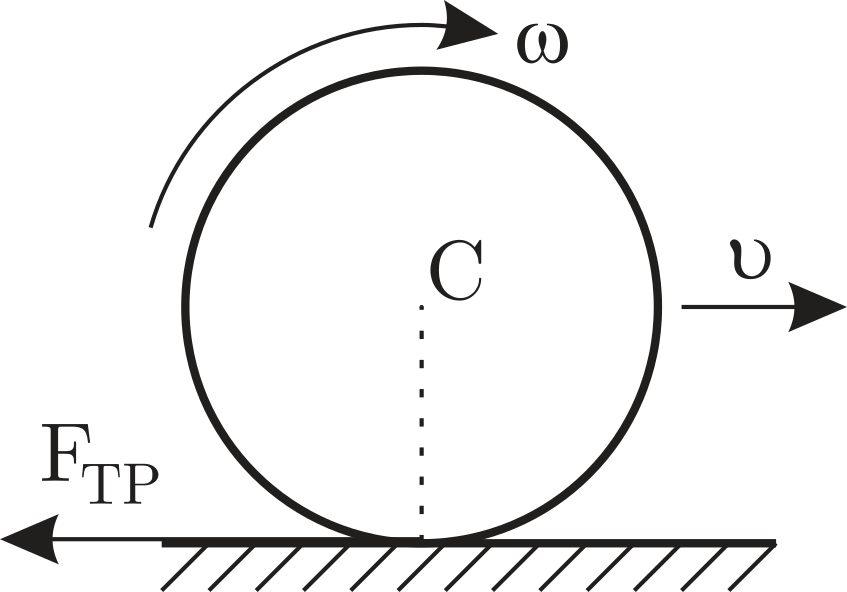
\includegraphics[width=0.72\textwidth]{E1_EN_assets/fig1.jpg}
    \caption{Figure 1.}
\end{figure}

Consequently, if only tangential friction force existed during rolling, then it would not be able to simultaneously reduce the translational and rotational speeds of the cylinder so that sliding would not occur. In reality, when the cylinder speed decreases, no slip occurs. This means that there is a moment of some other force, which is directed towards the moment of the friction force. It exceeds it in size and slows down the rotation of the cylinder so that slipping does not occur (Fig. 2). This is the moment of rolling friction force.

\begin{figure}[H]
    \centering
    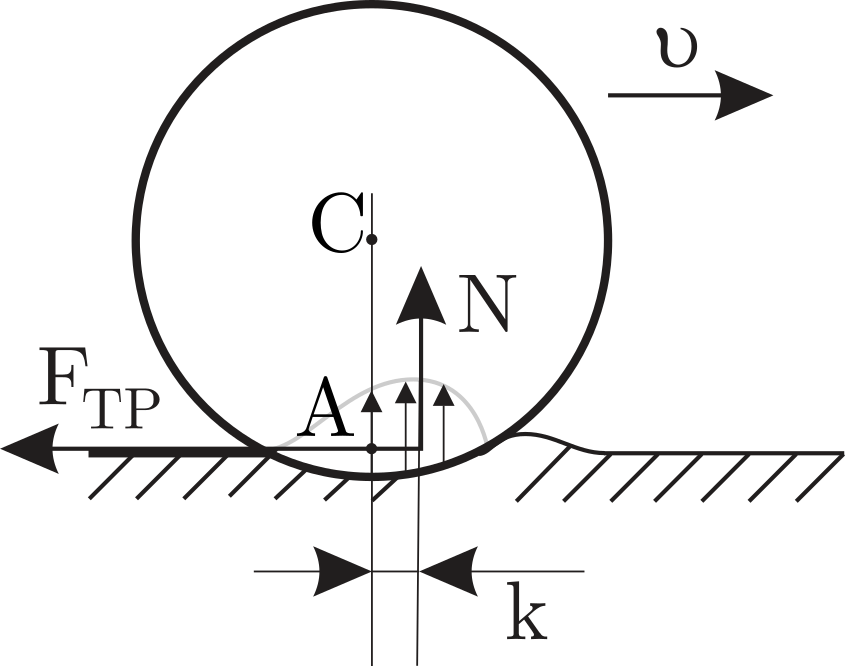
\includegraphics[width=0.72\textwidth]{E1_EN_assets/fig2.jpg}
    \caption{Figure 2.}
\end{figure}

The moment $M$ (relative to point $A$) of the rolling friction force is proportional to the force of the normal reaction of the support $N$, equal in modulus to the force of gravity: $$M = kN.$$ Постоянная величина $k$ называется коэффициентом трения качения. Момент сил трения качения всегда направлен так, чтобы уменьшать скорость вращения цилиндра. Следует отметить, что горизонтальная сила трения $F_\text{tr}$ приложена к цилиндру в точке касания с плоскостью, имеющей нулевую скорость. Поэтому сила $F_\text{tr}$ does not perform mechanical work.

\problembox{A1}{Determine experimentally the rolling friction coefficient $k$ of a cylinder rolling on a wooden block. Describe the measurement method and sketch the installation diagram.}{11.00}

\problembox{A2}{Determine experimentally the sliding friction coefficient $\mu$ of a cardboard cylinder on a tree. Give the measurement method and installation diagram.}{4.00}

Equipment: cylinder, protractor, adhesive mass, 50 cm ruler, block, white A4 sheet (2 pcs).

\vspace{1em}
\noindent\textit{Source:} \url{https://pho.rs/p/72}

\end{document}